\chapter{Projekt Aplikacji}
\section{Opis}
Aplikacja stworzona na potrzeby przeprowadzenia badań jest serwisem typu \textsl{RESTful}. Celem jest przechowywanie danych w bazie w postaci klucz-wartość.  Aplikacja udostępnia w tym celu \textsl{API}. Aby móc skorzystać z aplikacji klient musi się autoryzować unikalnym kluczem (\textsl{API key}). Klient posiadający klucz ma możliwość zapisywać i odczytywać dane. 

Klucz można otrzymać automatycznie wykonując żądanie: \textsl{GET /api/}. W odpowiedzi aplikacja zwróci unikalny, losowy klucz identyfikujący danego klienta. Do generowania kluczy użyty został mechanizm \textsl{UUID} (ang. \textsl{universally unique identifier}) generujący losowy 128 bitowy ciąg znaków. Przykładowy identyfikator wygląda następująco: \textsl{f0778bae-2902-4ff6-93fa-9776403ecb0f}.

Klient posiadający swój klucz może tworzyć, aktualizować, usuwać i pobierać wartości które są zapisane w bazie danych. Każde żądanie w adresie musi w adresie zawierać ten klucz. Początek żądania ma formę \textsl{/api/\{api\_key\}/}. W przypadku podania błędnego klucza lub jego braku aplikacja zwróci błąd autoryzacji. W tabeli \ref{tab:restcache-api} zostały zaprezentowane dostępne metody, do zarządzania danymi.
\begin{table}[!htb]
\centering
\caption{Metody dostępne w API aplikacji dla klienta}
\label{tab:restcache-api}
\begin{tabularx}{\textwidth}{@{} X X @{}}
\toprule
\multicolumn{1}{c}{\textbf{Żądanie HTTP}}            & \multicolumn{1}{c}{\textbf{Krótki opis}}                                               \\ \midrule
GET /api/\{api\_key\}/\{key\}                        & Pobranie obiektu z bazy znajdującego się pod kluczem \textsl\{key\}                   \\
POST /api/\{api\_key\}/\{key\}                       & Utworzenie obiektu w bazie pod kluczem \textsl\{key\}                                 \\
PUT /api/\{api\_key\}/\{key\}                        & Aktualizowanie obiektu w bazie, znajdującego się pod kluczem \textsl\{key\}        \\
DELETE /api/\{api\_key\}/\{key\} & Usunięcie elementu z bazy elementu o kluczu \textsl\{key\}                            \\
GET /api/\{api\_key\}                                & Pobranie wszystkich obiektów zapisanych w bazie, przypisanych kluczowi \textsl\{API\} \\
\end{tabularx}
\end{table}

Każda z metod służąca do modyfikowania danych ma zaimplementowane odpowiednie walidacje. Meetoda \textsl{} pozwala na pobranie zapisanej wartości w bazie danych. Jeśli nie istnieje wartość o podanym kluczu zwracany jest błąd \textsl{HTTP 404 - Not Found}. Następną metodą umożliwia tworzyć obiekty w bazie danych. Jeśli w bazie istnieje już obiekt o podanym kluczu, przypisany temu samemu klientowi aplikacja zwraca błąd \textsl{HTTP 409 - Conflict}.f

Ostatnią dostępną metodą jest żądanie \textsl{GET /api/\{api\_key\}}, które pozwala na pobranie wszystkich elementów z bazy danych. Je

Model wykorzystywany w aplikacji składa z dwóch klas które są jednakowo odwzorowane w kolekcjach bazy \textsl{MongoDB}. Klasa \textsl{Api} służy do przechowywania w bazie danych informacji o zarejestrowanych kluczach API (\textsl{API key}). Jeśli w kolekcji \textsl{Api} nie występuje klucz, aplikacja będzie zgłaszać błąd braku autoryzacji. Druga klasa, \textsl{Cache}, jest obiektem służącym do przechowywania.

Na rysunku \ref{fig:class_diagram} przedstawiony jest diagram klas aplikacji. 
\begin{figure}[!ht]
\centering
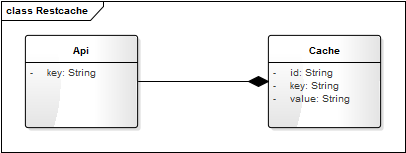
\includegraphics[width=13cm]{\ImgPath/diagram_klas.png}
\caption{Diagram klas aplikacji wykorzystywanej do przeprowadzenia testów}
\label{fig:class_diagram}
\end{figure}

\subsection{Infrastruktura}
Do przeprowadzenia testów wydajnościowych wykorzystywane były 3 serwery wirtualne. Specyfikacje techniczne serwerów wirtualnych, wykorzystanych w testach to: 
\begin{itemize}
    \item 8 rdzeni, 16 gigabajtów pamięci RAM, 160 gigabajtów dysku SSD dla serwera aplikacyjnego
    \item 4 rdzenie, 8 gigabajtów pamięci RAM, 80 gigabajtów dysku SSD dla serwera bazy danych 
    \item 4 rdzenie, 8 gigabajtów pamięci RAM, 80 gigabajtów dysku SSD dla serwera, na którym uruchomiony był program \textsl{Apache JMeter}
\end{itemize}
Serwery komunikowały się po sieci lokalnej (ang. \textsl{LAN}) bezpośrednio między sobą.

Na rysunku \ref{fig:deployment_diagram} zaprezentowany został diagram wdrożenia infrastruktury wykorzystanej do przeprowadzenia testóœ.
\begin{figure}[!ht]
\centering
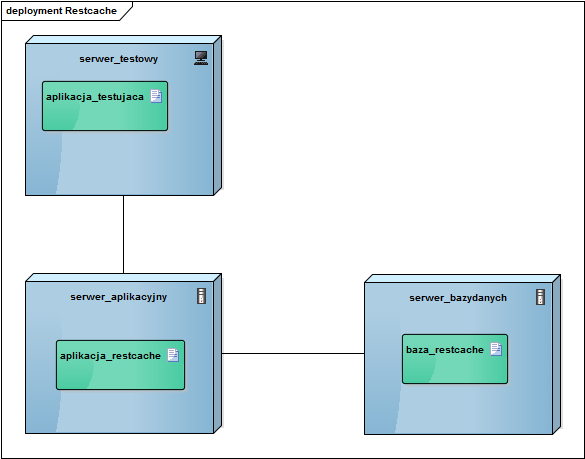
\includegraphics[width=13cm]{\ImgPath/diagram_wdrozenia.png}
\caption{Diagram wdrożenia infrastruktury wykorzystywanej do przeprowadzenia testów}
\label{fig:deployment_diagram}
\end{figure}

\subsection{Testy akceptacyjne} 

By potwierdzić, że \textsl{API} aplikacji w językach \textsl{Java} i \textsl{Go} jest zachowuje się tak samo zostało przygotowane 24 testy akceptacyjnych używając biblioteki \textsl{Spock}. 

W dodatku \ref{sec:acceptance_tests_appendix} przedstawione zostały rezultaty testów aplikacji uruchomionej na serwerze \textsl{Tomcat} (rysunek \ref{fig:acceptance_test_tomcat}), \textsl{Jetty} (rysunek \ref{fig:acceptance_test_jetty}) oraz w języku \textsl{Go} (rysunek \ref{fig:acceptance_test_go}).

